%% 
%% Copyright 2019-2020 Elsevier Ltd
%% 
%% This file is part of the 'CAS Bundle'.
%% --------------------------------------
%% 
%% It may be distributed under the conditions of the LaTeX Project Public
%% License, either version 1.2 of this license or (at your option) any
%% later version.  The latest version of this license is in
%%    http://www.latex-project.org/lppl.txt
%% and version 1.2 or later is part of all distributions of LaTeX
%% version 1999/12/01 or later.
%% 
%% The list of all files belonging to the 'CAS Bundle' is
%% given in the file `manifest.txt'.
%% 
%% Template article for cas-sc documentclass for 
%% double column output.

%\documentclass[a4paper,fleqn,longmktitle]{cas-sc}
\documentclass[a4paper,fleqn]{cas-sc}

% \usepackage[numbers]{natbib}
\usepackage[authoryear]{natbib}
%\usepackage[authoryear,longnamesfirst]{natbib}
\usepackage[export]{adjustbox}

%%%Author definitions
\def\tsc#1{\csdef{#1}{\textsc{\lowercase{#1}}\xspace}}
\tsc{WGM}
\tsc{QE}
\tsc{EP}
\tsc{PMS}
\tsc{BEC}
\tsc{DE}
%%%

\begin{document}
\let\WriteBookmarks\relax
\def\floatpagepagefraction{1}
\def\textpagefraction{.001}

% Short title
\shorttitle{Implementing adaptive operating policies to achieve economic, and groundwater sustainability goals in agriculture}

% Short author
\shortauthors{Rodríguez-Flores et~al.}

% Main title of the paper
\title [mode = title]{Implementing adaptive operating policies to achieve economic, and groundwater sustainability goals in agriculture using Evolutionary Multi-Objective Direct Policy Search}                      

\author[1]{José M. Rodríguez-Flores}[]
% Corresponding author indication
\cormark[1]
% Email id of the first author
\ead{jrodriguezflores3@ucmerced.edu}
\affiliation[1]{organization={Environmental Systems Program, University of California Merced},
    state={CA},
    country={USA}}
%  Credit authorship
\credit{Conceptualization of this study, Methodology, Software}

% Address/affiliation
% Second author
\author[2]{Rohini S. Gupta}[]
\affiliation[2]{organization={Department of Civil and Environmental Engineering, Cornell University},
    state={NY},
    country={USA}}
    
% Third author
\author[3]{Harrison B. Zeff}[]
\credit{Data curation, Writing - Original draft preparation}
% Address/affiliation
\affiliation[3]{organization={Department of Environmental Sciences and Engineering, University of North Carolina at Chapel Hill},
    state={NC},
    country={US}}
% Fourth author
\author[2]{Patrick M. Reed}[]
\credit{Data curation, Writing - Original draft preparation}
% Fifth author
\author[1]{Josué Medellín-Azuara}[]
\credit{Data curation, Writing - Original draft preparation}

% Corresponding author text
\cortext[cor1]{Corresponding author}

% Here goes the abstract
\begin{abstract}
Increasing irrigation demand has heavily relied on groundwater use, especially in places with highly variable water supplies that are vulnerable to drought. Groundwater management in agriculture is becoming increasingly challenging given the growing effects from overdraft and groundwater depletion worldwide. However, multiple challenges emerge when seeking to develop sustainable groundwater management in irrigated systems, such as trade-offs between the economic revenues from food production and groundwater resources, as well as the broad array of uncertainties in food-water systems. In this study we explore the applicability of Evolutionary Multi-Objective Direct Policy Search (EMODPS) to identify adaptive irrigation policies that water agencies and farmers can implement including operational decisions related to land use and groundwater use controls and a groundwater pumping fee. The EMODPS framework yields state-aware, adaptive policies that respond dynamically as system state conditions change, for example with variable surface water (e.g. shifting management strategies across wet versus dry years). For this study, we focus on the Semitropic Water Storage district located in the San Joaquin Valley, California to provide broader insights relevant to ongoing efforts to improve groundwater sustainability in the state. Our findings demonstrate that the adaptive irrigation policies can achieve a flexible groundwater management in a wide range of uncertain future scenarios while meeting sustainability objectives. Among these decisions pumping restrictions and reductions in inflexible irrigation demands from tree crops are actions that can support dry-year pumping while maximizing groundwater storage recovery during wet years. Policies suggest that an adaptive pumping fee is the most flexible decision to control groundwater pumping and land use. 

\end{abstract}

% Use if graphical abstract is present
% \begin{graphicalabstract}
% 
\includegraphics{figs/grabs.pdf}
% \end{graphicalabstract}

% Research highlights
\begin{highlights}
\item Research highlights item 1
\item Research highlights item 2
\item Research highlights item 3
\end{highlights}

% Keywords
% Each keyword is seperated by \sep
\begin{keywords}
quadrupole exciton \sep polariton \sep \WGM \sep \BEC
\end{keywords}


\maketitle

\section{Introduction}

As irrigation water demand increases due to increased crop acreage and droughts become more frequent, agricultural regions in the world are relying more on groundwater to make up for surface water losses. In Mediterranean climate regions, such as California, groundwater is the primary water source for buffering drought impacts and food production \citep{malmgren_groundwater_2022,priyan_issues_2021}. Aquifer systems’ dynamics are sensitive to changes in temperature, precipitation, and surface water flows, that can be directly impacted by climate change \citep{cuthbert_global_2019,wu_divergent_2020}. However, one of the largest impacts from climate change are the resulting adaptation driven changes in land use and shifting water demands from human activities \citep{taylor_ground_2013}. Globally, groundwater provides 43 percent of the total irrigation needs \citep{siebert_groundwater_2010}, and its share is expected to increase as surface water scarcity increases \citep{wada_nonsustainable_2012}. In California, the limits in coordinated and regulated groundwater management in irrigation-based agriculture have led to decades of increasing stress and depletion of the state's aquifers \citep{vasco_satellite-based_2019}, affecting dependent ecosystems \citep{bierkens_non-renewable_2019}, limiting its access to shallow water-table reliant communities \citep{pauloo_domestic_2020,perrone_dry_2017}, increasing land subsidence \citep{smith_groundwater_2020}, reducing groundwater storage and storativity \citep{alam_post-drought_2021}, and degradation of water quality \citep{levy_critical_2021}. 

The largest rate of groundwater depletion in California has been observed in the San Joaquin Valley (SJV) \citep{ojha_sustained_2018}. The SJV is the most important agricultural region in the United States by economic value \citep{usda_national_2020}, but also strongly susceptible to drought risk. Most of the region’s snowpack and water supply comes from limited atmospheric-river driven events \citep{espinoza_global_2018}. Increasing temperatures and evapotranspiration linked to a warming climate are expected to further reduce snowpack runoff and surface water supply \citep{fernandez-bou_regional_2021,vahmani_will_2022}. Additionally, human factors such as increasing irrigation demand can exacerbate vulnerabilities to increasingly intense droughts \citep{he_intensification_2017}. Over the past decade, the agricultural sector has been significantly impacted by multi-year droughts \citep{lund_lessons_2018,medellin-azuara_economic_2022}. Groundwater pumping is used as a buffer to reduce the negative impacts to agricultural production from surface water shortages, but increasing pumping and a lack of coordinated management have led to significant declines in groundwater levels and reductions in the regional aquifer's capacity to recover \citep{liu_groundwater_2022}.  Additionally, the SJV has seen a significant expansion of perennial tree crops, mainly almonds, which is the most important commodity by value in the region \citep{usda_national_2020}. Although highly profitable, the expansion of perennial tree crops represents a less flexible water demand and a higher financial risk to water shortages due to high establishment costs \citep{mall_water_2019,qin_flexibility_2019}.   

Given the consequences from overdraft in California, the 2014 Sustainable Groundwater Management Act (SGMA) \citep{dwr_sustainable_2021} was put in place to require critically over-drafted basins to achieve sustainability in terms of balancing their recharge and extraction by 2040. Groundwater Sustainability Agencies (GSAs) are locally formed agencies responsible for developing and enforcing policies to manage water conjunctively to address groundwater sustainability. The state defined guidelines in the Sustainable Management Criteria \citep{dwr_sustainable_2017} that GSAs can use to develop management strategies to achieve sustainable goals, including sustainable groundwater levels. The sustainable criteria define a margin of operational flexibility where the groundwater depth can go above the measurable objective (henceforth referred as SGMA objective) but not above the minimum threshold where undesirable results (e.g., dry wells) may occur (Figure 1). Within this framework, GSAs can develop flexible groundwater management strategies, allowing pumping during dry years and maximizing groundwater recovery during wet years. Overall, California's food production needs to adapt operational water and land allocation decisions and crop choice to achieve groundwater sustainability goals and be less vulnerable to surface water shortages. 


 \begin{figure}[ht]
    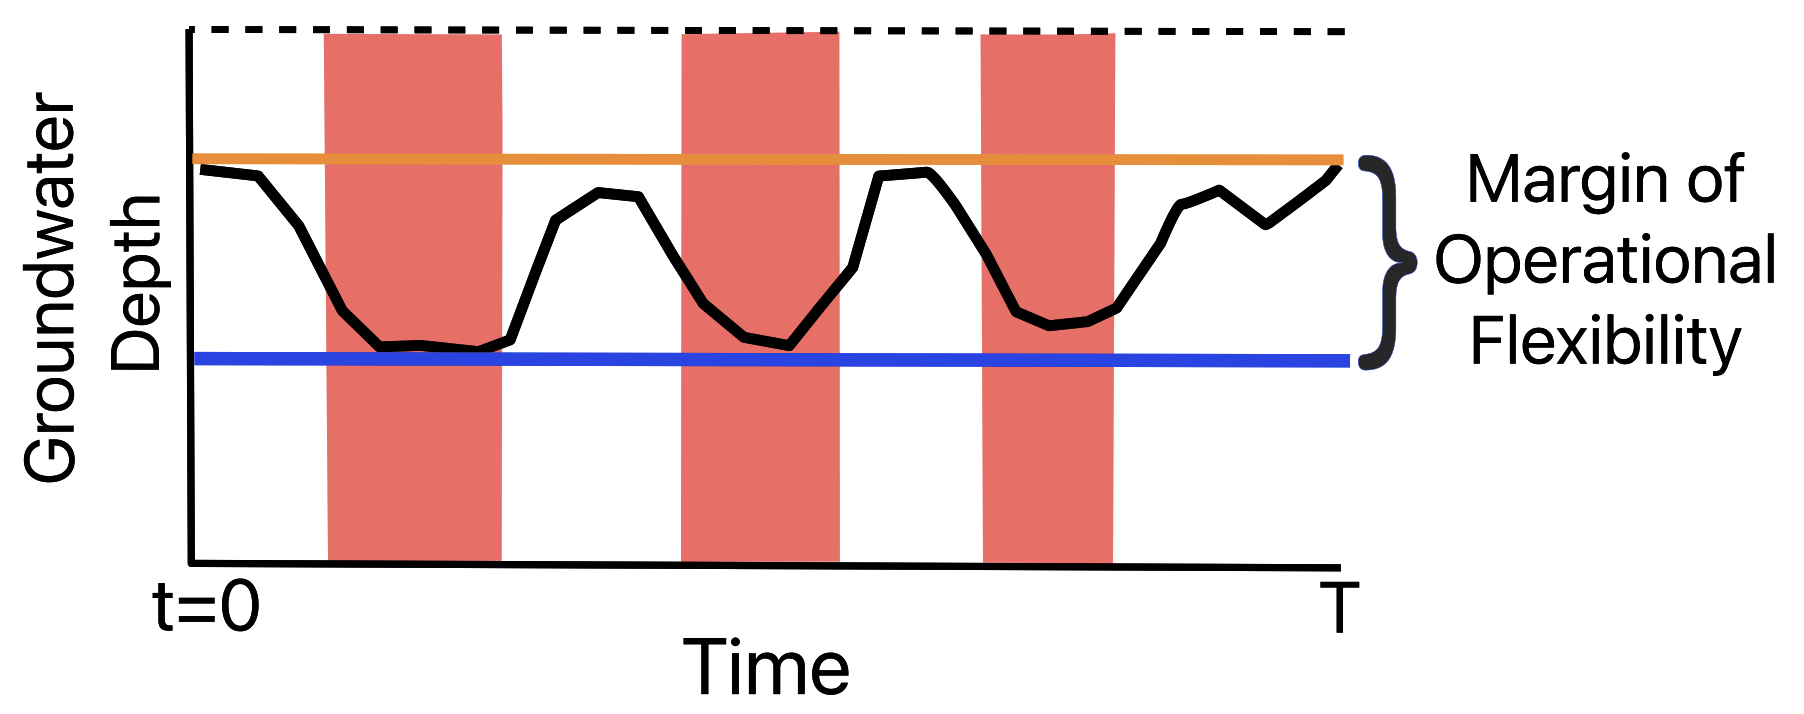
\includegraphics[width=0.5\textwidth,center]{conceptual_sgma_policy.jpg}
    \caption{Conceptual behavior of groundwater depth under sustainable management. Dashed line represents the reference ground surface level, orange line depicts the measurable objective (SGMA objective) and blue line represents the minimum threshold. Red rectangles depict dry periods when groundwater depth increases.}
    \label{fig:1}
\end{figure}

Multiple challenges that are inherent to coupled food-water systems \citep{polhill_modelling_2016} impact the development of groundwater management policies in the SJV. First, food-water systems are dynamic, where each component can evolve and lead to feed-backs \citep{filatova_regime_2016}. Thus, management decisions need to adapt as the coupled system evolves. Second, water management policies may result in trade-offs between economic and sustainability objectives \citep{mcdermid_minimizing_2021,stone_economic_2022,torhan_tradeoffs_2022,null_pareto_2021}. Lastly, there are intrinsic deep uncertainties \citep{stirling_keep_2010} that need to be considered to implement robust policies, including uncertain surface water supplies and crop prices. There is a growing base of literature focused on assessing management policies and mechanisms for groundwater sustainability in agriculture. Water and land use controls as well as economic instruments are the most common strategies that have been implemented. Examples of these mechanisms are groundwater pumping taxing and pricing  \citep{madani_exogenous_2013,mulligan_assessing_2014,stone_economic_2022,wang_development_2023}, pumping restrictions \citep{young_hydrologic-economic_2021,lan_performance_2021,macewan_hydroeconomic_2017,rodriguez-flores_global_2022,wang_development_2023}, pricing energy \citep{hrozencik_impacts_2022}, groundwater markets or water trading mechanisms \citep{khan_effect_2019,kuwayama_regulation_2013,safari_market-based_2023}, land fallowing \citep{van_schmidt_linkages_2022} and land management \citep{bourque_balancing_2019,li_evaluation_2018,bryant_shaping_2020}, implemented individually or utilized in conjunction \citep{graveline_combining_2020,hrozencik_heterogeneous_2017}. However, most of these studies do not capture the complexity of actually implementing these mechanisms in decision making. For example, they do not take into account intrinsic uncertainties such as annual variability in surface water supplies and the trade-offs between groundwater sustainability objectives and economic revenues. 

Secondly, finding optimal groundwater management policies is a nontrivial task. Most formulations to do so are characterized by non-linearity and non-convexity, and must consider a broad array of objectives that balance trade-offs across groundwater sustainability agencies and farmers (i.e., maximizing economic revenues and minimizing distance to groundwater). Heuristic methods such as  multi-objective evolutionary algorithms (MOEAs) has been demonstrated in their ability to address these complexities and discover high quality approximations of optimal trade-offs among objectives in the Pareto-front \citep{reed_evolutionary_2013}. Thus, the resulting Pareto optimal approximate set of solutions are those where there is not a solution with a better performance of an objective without degrading the performance in the remaining objectives \citep{coello_evolutionary_2007}. Even though heuristic optimization frameworks hold promise for support decision making in agriculture \citep{memmah_metaheuristics_2015}, there are few applications pertaining to larger and more complex inter-connected food-water systems. Prior studies show the applicability of MOEAs in groundwater use controls \citep{afshar_multi-objective_2020,salehi_shafa_multi-objective_2023,habibi_davijani_optimization_2016,mehrabi_assessment_2021,banihabib_development_2019,hesamfar_simulation-based_2023} and this study expands the application of MOEAs to find coordinated optimal land and water use decisions to achieve groundwater sustainability and economic objectives in agriculture.  

As reviewed by \citet{thomann_adaptive_2020}, there is a need for new groundwater management frameworks that are dynamic and adaptively responsive to changes in observed system changes. In this study, we draw on Direct Policy Search (DPS) introduced by \citet{rosenstein_robot_2001} as a parameterization-simulation-optimization formulation where in a control policy is parameterized using non-linear universal functions as neural networks and radial basis functions. In DPS, the parameters of the control policy function are optimized rather than the decisions themselves using a simulation-optimization process to search for optimal operations for a system. The application of DPS to water systems was introduced by \citet{koutsoyiannis_evaluation_2003} in reservoir operations and subsequently extended Evolutionary Multi-objective Direct Policy Search (EMODPS) formalized by \citet{giuliani_coupled_2016}. As reviewed by \citet{giul}This modeling framework has proven capable of discovering optimal dynamic adaptive policies in complex decision making under uncertainty in water systems \citep{macian-sorribes_inferring_2019} with multiple applications in reservoir operation and financial portfolios \citep{gupta_can_2020,zatarain_salazar_balancing_2017,hamilton_stream_2022}. Additionally, EMODPS can reduce the "curse of dimensionality" of other dynamic frameworks as Stochastic Dynamic Programming applied in agriculture \citep{taylor_dynamic_1993}. 

In this study we formulate a 5-objective application of EMODPS where resulting control policies can map current states of system variables (e.g surface water available, groundwater depth and irrigation demand) to adaptively inform decisions, such as pumping and land use controls as well as pricing pumping, that should be made in a given year at the GSA level. The resultant Pareto set of solutions represent a control policy that can be implemented to optimize the objectives: maximize revenue from food production, minimize distance to groundwater (groundwater depth), maximize minimum economic revenue, minimize maximum groundwater depth change and maximize the number of years the groundwater level is at the measurable objective. Through a Robust Decision Making (RDM) (\citep{groves_robust_2019,lempert_making_2013}) framework, solutions are then assessed to find the policies that perform well under multiple system state conditions or states of the world (SOWs). RDM has been used to assess the ability of water management polices to address water demand, economic and sustainability objectives under uncertainty (\citep{graveline_combining_2020,huskova_screening_2016,miro_adaptive_2021,hadjimichael_defining_2020,shuai_robust_2022}). Building off these examples we identify robust policies that achieve expected performances in groundwater depth and economic revenues at the GSA level and that also meet the Sustainable Management Criteria. 

This study further demonstrates a novel application of a combined hydro-economic and heuristic methods using a bi-level optimization process where an agricultural production model with a groundwater depth response function is nested the MOEA to find adaptive management policies to achieve groundwater sustainability. This modeling framework is applied to the Semitropic Water Storage District GSA, which represents a broad set groundwater sustainability agencies in the San Joaquin Valley. The objectives of this study are twofold:  

\begin{enumerate}
    \item  Use EMODPS to identify adaptive strategies that achieve groundwater sustainability and economic goals accounting for the characteristics of the food-water system. 
    
    \item Assess the performance of the optimal policies within the context of the sustainable groundwater management criteria defined by the state.
\end{enumerate}

\section{Study area}


The study area of this research is the Semitropic Water Storage District (SWSD), located in the SJV and the Kern County groundwater basin (Figure 2). The SWSD also operates its own Groundwater Sustainability Agency, which  determines strategies that can be implemented depending on the water budget of each year. Four possible strategies are analyzed in this study: (1) a groundwater use control and a (2) groundwater pumping fee that is implemented by the GSA. Further, we also implement decisions pertaining to farmers’ land management: (3) total land use control and (4) perennial crops planting restriction. Other management strategies such as water market mechanisms and supply-side policies focused on augmenting groundwater storage, as managed aquifer recharge (\citep{ulibarri_assessing_2021}), are out of the scope of this study. As other regions in the SJV the expansion of almonds and other perennial crops has been observed in the past 10 years. Other important commodities in the district include vines, alfalfa, corn, cotton, and cucumbers shown in Figure S1 in the Supplemental Information (SI). 
  

\begin{figure}[H]
    \centering
    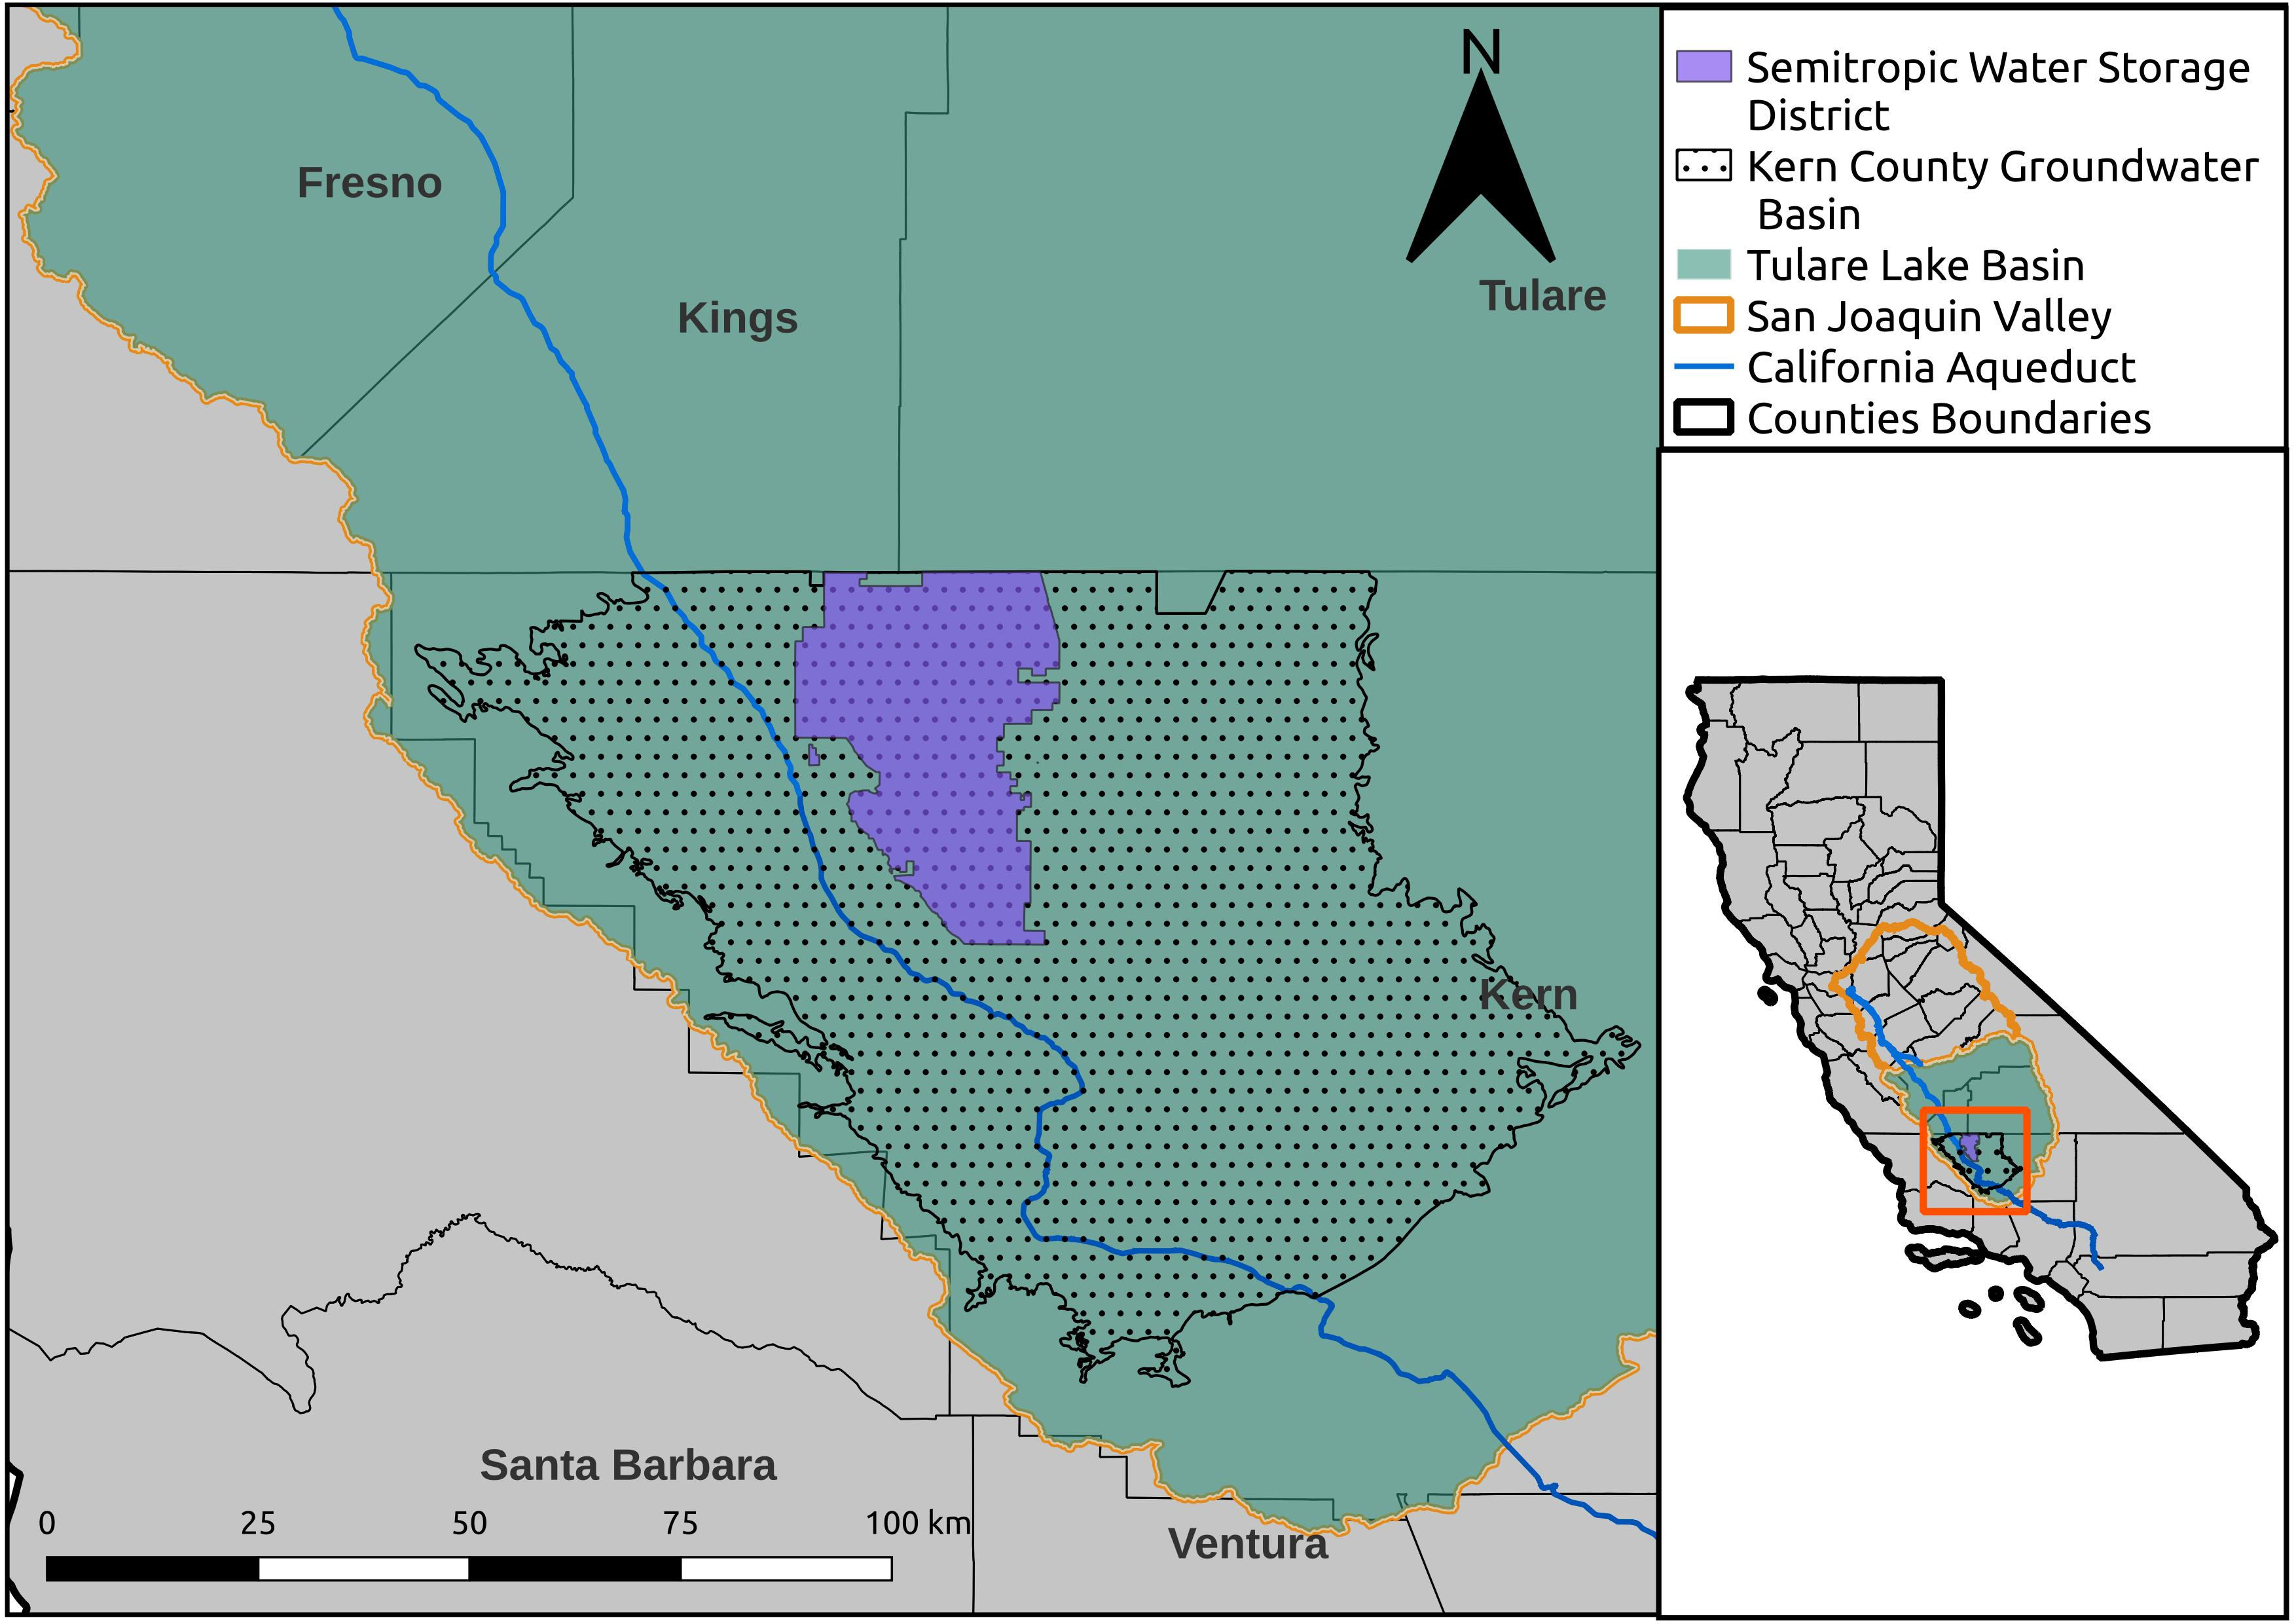
\includegraphics[width=0.8\textwidth]{Map_Semitropic.jpg}
    \caption{Semitropic Water Storage District study area located in the California’s San Joaquin Valley.}
    \label{fig:1}
\end{figure}

\subsection{Semitropic GSA Hydro-Economic model}

In food-water systems Hydro-Economic Models have been used as decision support modeling tools to assess water policy and climate change adaptation decisions (\citep{ward_hydroeconomic_2021,harou_hydro-economic_2009}). HEMs are able to abstract stakeholders decisions (e.g farmers) and hydrology dynamics, as well as their feedback, by integrating economic models with hydrological response functions (\citep{harou_hydro-economic_2009}). Given the modular characteristic of these coupled modeling methods is possible to assess the performance of economic revenues and aquifer dynamics, as shown by \textcite{macewan_hydroeconomic_2017}, \textcite{afshar_multi-objective_2020}, \textcite{rodriguez-flores_global_2022} and \textcite{graveline_combining_2020}. Additionally, these methods are flexible to assess the performance of water management policies, under different climate scenarios, and spatial and time scales.


The Elsevier cas-sc class is based on the
standard article class and supports almost all of the functionality of
that class. In addition, it features commands and options to format the
\begin{itemize} \item document style \item baselineskip \item front
matter \item keywords and MSC codes \item theorems, definitions and
proofs \item lables of enumerations \item citation style and labeling.
\end{itemize}

This class depends on the following packages
for its proper functioning:

\begin{enumerate}
\itemsep=0pt
\item {natbib.sty} for citation processing;
\item {geometry.sty} for margin settings;
\item {fleqn.clo} for left aligned equations;
\item {graphicx.sty} for graphics inclusion;
\item {hyperref.sty} optional packages if hyperlinking is
  required in the document;
\end{enumerate}  

All the above packages are part of any
standard \LaTeX{} installation.
Therefore, the users need not be
bothered about downloading any extra packages.

\section{Installation}

The package is available at author resources page at Elsevier
(\url{http://www.elsevier.com/locate/latex}).
The class may be moved or copied to a place, usually,\linebreak
\verb+$TEXMF/tex/latex/elsevier/+, %$%%%%%%%%%%%%%%%%%%%%%%%%%%%%
or a folder which will be read                   
by \LaTeX{} during document compilation.  The \TeX{} file
database needs updation after moving/copying class file.  Usually,
we use commands like \verb+mktexlsr+ or \verb+texhash+ depending
upon the distribution and operating system.

\section{Front matter}

The author names and affiliations could be formatted in two ways:
\begin{enumerate}[(1)]
\item Group the authors per affiliation.
\item Use footnotes to indicate the affiliations.
\end{enumerate}
See the front matter of this document for examples. 
You are recommended to conform your choice to the journal you 
are submitting to.

\section{Bibliography styles}

There are various bibliography styles available. You can select the
style of your choice in the preamble of this document. These styles are
Elsevier styles based on standard styles like Harvard and Vancouver.
Please use Bib\TeX\ to generate your bibliography and include DOIs
whenever available.

Here are two sample references: \citep{Fortunato2010}
\citep{Fortunato2010,NewmanGirvan2004}
\citep{Fortunato2010,Vehlowetal2013}

\section{Floats}
{Figures} may be included using the command,\linebreak 
\verb+\includegraphics+ in
combination with or without its several options to further control
graphic. \verb+\includegraphics+ is provided by {graphic[s,x].sty}
which is part of any standard \LaTeX{} distribution.
{graphicx.sty} is loaded by default. \LaTeX{} accepts figures in
the postscript format while pdf\LaTeX{} accepts {*.pdf},
{*.mps} (metapost), {*.jpg} and {*.png} formats. 
pdf\LaTeX{} does not accept graphic files in the postscript format. 

\begin{figure}
	\centering
		
\includegraphics[scale=.75]{figs/Fig1.pdf}
	\caption{The evanescent light - $1S$ quadrupole coupling
	($g_{1,l}$) scaled to the bulk exciton-photon coupling
	($g_{1,2}$). The size parameter $kr_{0}$ is denoted as $x$ and
	the \PMS is placed directly on the cuprous oxide sample ($\delta
	r=0$, See also Table \protect\ref{tbl1}).}
	\label{FIG:1}
\end{figure}


The \verb+table+ environment is handy for marking up tabular
material. If users want to use {multirow.sty},
{array.sty}, etc., to fine control/enhance the tables, they
are welcome to load any package of their choice and
{cas-sc.cls} will work in combination with all loaded
packages.

\begin{table}[width=.9\linewidth,cols=4,pos=h]
\caption{This is a test caption. This is a test caption. This is a test
caption. This is a test caption.}\label{tbl1}
\begin{tabular*}{\tblwidth}{@{} LLLL@{} }
\toprule
Col 1 & Col 2 & Col 3 & Col4\\
\midrule
12345 & 12345 & 123 & 12345 \\
12345 & 12345 & 123 & 12345 \\
12345 & 12345 & 123 & 12345 \\
12345 & 12345 & 123 & 12345 \\
12345 & 12345 & 123 & 12345 \\
\bottomrule
\end{tabular*}
\end{table}

\section[Theorem and ...]{Theorem and theorem like environments}

{cas-sc.cls} provides a few shortcuts to format theorems and
theorem-like environments with ease. In all commands the options that
are used with the \verb+\newtheorem+ command will work exactly in the same
manner. {cas-sc.cls} provides three commands to format theorem or
theorem-like environments: 

\begin{verbatim}
 \newtheorem{theorem}{Theorem}
 \newtheorem{lemma}[theorem]{Lemma}
 \newdefinition{rmk}{Remark}
 \newproof{pf}{Proof}
 \newproof{pot}{Proof of Theorem \ref{thm2}}
\end{verbatim}


The \verb+\newtheorem+ command formats a
theorem in \LaTeX's default style with italicized font, bold font
for theorem heading and theorem number at the right hand side of the
theorem heading.  It also optionally accepts an argument which
will be printed as an extra heading in parentheses. 

\begin{verbatim}
  \begin{theorem} 
   For system (8), consensus can be achieved with 
   $\|T_{\omega z}$ ...
     \begin{eqnarray}\label{10}
     ....
     \end{eqnarray}
  \end{theorem}
\end{verbatim}  


\newtheorem{theorem}{Theorem}

\begin{theorem}
For system (8), consensus can be achieved with 
$\|T_{\omega z}$ ...
\begin{eqnarray}\label{10}
....
\end{eqnarray}
\end{theorem}

The \verb+\newdefinition+ command is the same in
all respects as its \verb+\newtheorem+ counterpart except that
the font shape is roman instead of italic.  Both
\verb+\newdefinition+ and \verb+\newtheorem+ commands
automatically define counters for the environments defined.

The \verb+\newproof+ command defines proof environments with
upright font shape.  No counters are defined. 


\section[Enumerated ...]{Enumerated and Itemized Lists}
{cas-sc.cls} provides an extended list processing macros
which makes the usage a bit more user friendly than the default
\LaTeX{} list macros.   With an optional argument to the
\verb+\begin{enumerate}+ command, you can change the list counter
type and its attributes.

\begin{verbatim}
 \begin{enumerate}[1.]
 \item The enumerate environment starts with an optional
   argument `1.', so that the item counter will be suffixed
   by a period.
 \item You can use `a)' for alphabetical counter and '(i)' 
  for roman counter.
  \begin{enumerate}[a)]
    \item Another level of list with alphabetical counter.
    \item One more item before we start another.
    \item One more item before we start another.
    \item One more item before we start another.
    \item One more item before we start another.
\end{verbatim}

Further, the enhanced list environment allows one to prefix a
string like `step' to all the item numbers.  

\begin{verbatim}
 \begin{enumerate}[Step 1.]
  \item This is the first step of the example list.
  \item Obviously this is the second step.
  \item The final step to wind up this example.
 \end{enumerate}
\end{verbatim}

\section{Cross-references}
In electronic publications, articles may be internally
hyperlinked. Hyperlinks are generated from proper
cross-references in the article.  For example, the words
\textcolor{black!80}{Fig.~1} will never be more than simple text,
whereas the proper cross-reference \verb+\ref{tiger}+ may be
turned into a hyperlink to the figure itself:
\textcolor{blue}{Fig.~1}.  In the same way,
the words \textcolor{blue}{Ref.~[1]} will fail to turn into a
hyperlink; the proper cross-reference is \verb+\citep{Knuth96}+.
Cross-referencing is possible in \LaTeX{} for sections,
subsections, formulae, figures, tables, and literature
references.

\section{Bibliography}

Two bibliographic style files (\verb+*.bst+) are provided ---
{model1-num-names.bst} and {model2-names.bst} --- the first one can be
used for the numbered scheme. This can also be used for the numbered
with new options of {natbib.sty}. The second one is for the author year
scheme. When  you use model2-names.bst, the citation commands will be
like \verb+\citepp+,  \verb+\citept+, \verb+\citealt+ etc. However when
you use model1-num-names.bst, you may use only \verb+\cite+ command.

\verb+thebibliography+ environment.  Each reference is a\linebreak
\verb+\bibitem+ and each \verb+\bibitem+ is identified by a label,
by which it can be cited in the text:

\noindent In connection with cross-referencing and
possible future hyperlinking it is not a good idea to collect
more that one literature item in one \verb+\bibitem+.  The
so-called Harvard or author-year style of referencing is enabled
by the \LaTeX{} package {natbib}. With this package the
literature can be cited as follows:

\begin{enumerate}[\textbullet]
\item Parenthetical: \verb+\citep{WB96}+ produces (Wettig \& Brown, 1996).
\item Textual: \verb+\citet{ESG96}+ produces Elson et al. (1996).
\item An affix and part of a reference:\break
\verb+\citep[e.g.][Ch. 2]{Gea97}+ produces (e.g. Governato et
al., 1997, Ch. 2).
\end{enumerate}

In the numbered scheme of citation, \verb+\cite{<label>}+ is used,
since \verb+\citep+ or \verb+\citet+ has no relevance in the numbered
scheme.  {natbib} package is loaded by {cas-sc} with
\verb+numbers+ as default option.  You can change this to author-year
or harvard scheme by adding option \verb+authoryear+ in the class
loading command.  If you want to use more options of the {natbib}
package, you can do so with the \verb+\biboptions+ command.  For
details of various options of the {natbib} package, please take a
look at the {natbib} documentation, which is part of any standard
\LaTeX{} installation.

\appendix
\section{My Appendix}
Appendix sections are coded under \verb+\appendix+.

\verb+\printcredits+ command is used after appendix sections to list 
author credit taxonomy contribution roles tagged using \verb+\credit+ 
in frontmatter.

\printcredits

%% Loading bibliography style file
% \bibliographystyle{model1-num-names}
\bibliographystyle{cas-model2-names}

% Loading bibliography database
\bibliography{Bio}

\end{document}

